\section{Register description}
\regover{
{\hyperref[dma-DMA-IntStatus]{DMA\_IntStatus}}&
\\
\hline
{\hyperref[dma-DMA-IntTCStatus]{DMA\_IntTCStatus}}&
\\
\hline
{\hyperref[dma-DMA-IntTCClear]{DMA\_IntTCClear}}&
\\
\hline
{\hyperref[dma-DMA-IntErrorStatus]{DMA\_IntErrorStatus}}&
\\
\hline
{\hyperref[dma-DMA-IntErrClr]{DMA\_IntErrClr}}&
\\
\hline
{\hyperref[dma-DMA-RawIntTCStatus]{DMA\_RawIntTCStatus}}&
\\
\hline
{\hyperref[dma-DMA-RawIntErrorStatus]{DMA\_RawIntErrorStatus}}&
\\
\hline
{\hyperref[dma-DMA-EnbldChns]{DMA\_EnbldChns}}&
\\
\hline
{\hyperref[dma-DMA-SoftBReq]{DMA\_SoftBReq}}&
\\
\hline
{\hyperref[dma-DMA-SoftSReq]{DMA\_SoftSReq}}&
\\
\hline
{\hyperref[dma-DMA-SoftLBReq]{DMA\_SoftLBReq}}&
\\
\hline
{\hyperref[dma-DMA-SoftLSReq]{DMA\_SoftLSReq}}&
\\
\hline
{\hyperref[dma-DMA-Config]{DMA\_Config}}&
\\
\hline
{\hyperref[dma-DMA-Sync]{DMA\_Sync}}&
\\
\hline
{\hyperref[dma-DMA-C0SrcAddr]{DMA\_C0SrcAddr}}&
\\
\hline
{\hyperref[dma-DMA-C0DstAddr]{DMA\_C0DstAddr}}&
\\
\hline
{\hyperref[dma-DMA-C0LLI]{DMA\_C0LLI}}&
\\
\hline
{\hyperref[dma-DMA-C0Control]{DMA\_C0Control}}&
\\
\hline
{\hyperref[dma-DMA-C0Config]{DMA\_C0Config}}&
\\
\hline
{\hyperref[dma-DMA-C0RSVD]{DMA\_C0RSVD}}&
\\
\hline
{\hyperref[dma-DMA-C1SrcAddr]{DMA\_C1SrcAddr}}&
\\
\hline
{\hyperref[dma-DMA-C1DstAddr]{DMA\_C1DstAddr}}&
\\
\hline
{\hyperref[dma-DMA-C1LLI]{DMA\_C1LLI}}&
\\
\hline
{\hyperref[dma-DMA-C1Control]{DMA\_C1Control}}&
\\
\hline
{\hyperref[dma-DMA-C1Config]{DMA\_C1Config}}&
\\
\hline
{\hyperref[dma-DMA-C1RSVD]{DMA\_C1RSVD}}&
\\
\hline
{\hyperref[dma-DMA-C2SrcAddr]{DMA\_C2SrcAddr}}&
\\
\hline
{\hyperref[dma-DMA-C2DstAddr]{DMA\_C2DstAddr}}&
\\
\hline
{\hyperref[dma-DMA-C2LLI]{DMA\_C2LLI}}&
\\
\hline
{\hyperref[dma-DMA-C2Control]{DMA\_C2Control}}&
\\
\hline
{\hyperref[dma-DMA-C2Config]{DMA\_C2Config}}&
\\
\hline
{\hyperref[dma-DMA-C2RSVD]{DMA\_C2RSVD}}&
\\
\hline
{\hyperref[dma-DMA-C3SrcAddr]{DMA\_C3SrcAddr}}&
\\
\hline
{\hyperref[dma-DMA-C3DstAddr]{DMA\_C3DstAddr}}&
\\
\hline
{\hyperref[dma-DMA-C3LLI]{DMA\_C3LLI}}&
\\
\hline
{\hyperref[dma-DMA-C3Control]{DMA\_C3Control}}&
\\
\hline
{\hyperref[dma-DMA-C3Config]{DMA\_C3Config}}&
\\
\hline
{\hyperref[dma-DMA-C3RSVD]{DMA\_C3RSVD}}&
\\
\hline
{\hyperref[dma-DMA-C4SrcAddr]{DMA\_C4SrcAddr}}&
\\
\hline
{\hyperref[dma-DMA-C4DstAddr]{DMA\_C4DstAddr}}&
\\
\hline
{\hyperref[dma-DMA-C4LLI]{DMA\_C4LLI}}&
\\
\hline
{\hyperref[dma-DMA-C4Control]{DMA\_C4Control}}&
\\
\hline
{\hyperref[dma-DMA-C4Config]{DMA\_C4Config}}&
\\
\hline
{\hyperref[dma-DMA-C4RSVD]{DMA\_C4RSVD}}&
\\
\hline
{\hyperref[dma-DMA-C5SrcAddr]{DMA\_C5SrcAddr}}&
\\
\hline
{\hyperref[dma-DMA-C5DstAddr]{DMA\_C5DstAddr}}&
\\
\hline
{\hyperref[dma-DMA-C5LLI]{DMA\_C5LLI}}&
\\
\hline
{\hyperref[dma-DMA-C5Control]{DMA\_C5Control}}&
\\
\hline
{\hyperref[dma-DMA-C5Config]{DMA\_C5Config}}&
\\
\hline
{\hyperref[dma-DMA-C5RSVD]{DMA\_C5RSVD}}&
\\
\hline
{\hyperref[dma-DMA-C6SrcAddr]{DMA\_C6SrcAddr}}&
\\
\hline
{\hyperref[dma-DMA-C6DstAddr]{DMA\_C6DstAddr}}&
\\
\hline
{\hyperref[dma-DMA-C6LLI]{DMA\_C6LLI}}&
\\
\hline
{\hyperref[dma-DMA-C6Control]{DMA\_C6Control}}&
\\
\hline
{\hyperref[dma-DMA-C6Config]{DMA\_C6Config}}&
\\
\hline
{\hyperref[dma-DMA-C6RSVD]{DMA\_C6RSVD}}&
\\
\hline
{\hyperref[dma-DMA-C7SrcAddr]{DMA\_C7SrcAddr}}&
\\
\hline
{\hyperref[dma-DMA-C7DstAddr]{DMA\_C7DstAddr}}&
\\
\hline
{\hyperref[dma-DMA-C7LLI]{DMA\_C7LLI}}&
\\
\hline
{\hyperref[dma-DMA-C7Control]{DMA\_C7Control}}&
\\
\hline
{\hyperref[dma-DMA-C7Config]{DMA\_C7Config}}&
\\
\hline
{\hyperref[dma-DMA-C7RSVD]{DMA\_C7RSVD}}&
\\
\hline
}

\subsection{DMA\_IntStatus}
\label{dma-DMA-IntStatus}
Address:0x2000c000
 \begin{figure}[H]
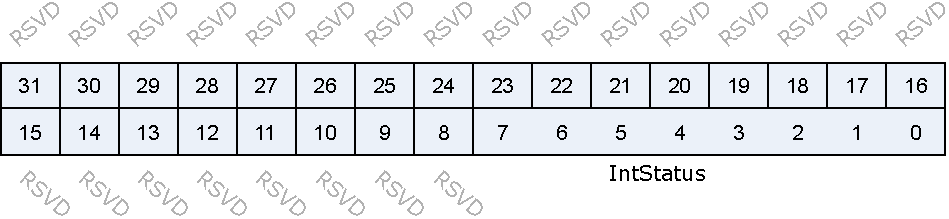
\includegraphics{dma_DMA_IntStatus.pdf}
\end{figure}

\regdes{31:8&RSVD& & & \\\hline
7:0&IntStatus&r&0&Status of the DMA interrupts after masking\\\hline

}
\subsection{DMA\_IntTCStatus}
\label{dma-DMA-IntTCStatus}
Address:0x2000c004
 \begin{figure}[H]
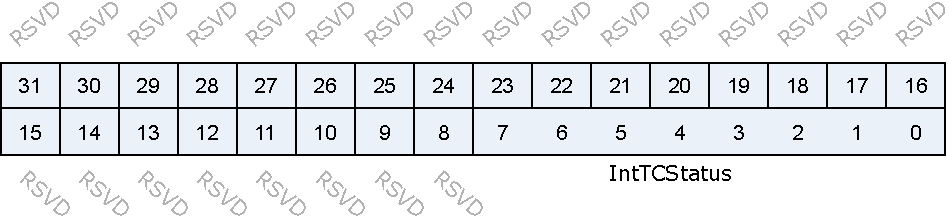
\includegraphics{dma_DMA_IntTCStatus.pdf}
\end{figure}

\regdes{31:8&RSVD& & & \\\hline
7:0&IntTCStatus&r&0&Interrupt terminal count request status\\\hline

}
\subsection{DMA\_IntTCClear}
\label{dma-DMA-IntTCClear}
Address:0x2000c008
 \begin{figure}[H]
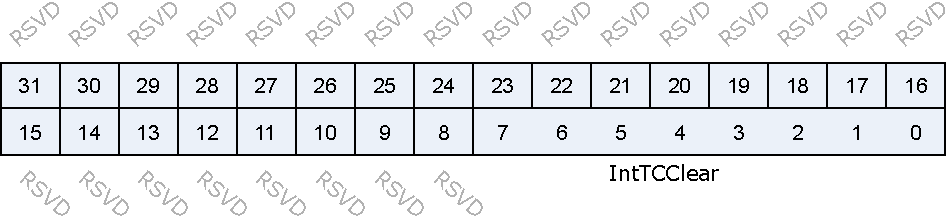
\includegraphics{dma_DMA_IntTCClear.pdf}
\end{figure}

\regdes{31:8&RSVD& & & \\\hline
7:0&IntTCClear&w&0&Terminal count request clear\\\hline

}
\subsection{DMA\_IntErrorStatus}
\label{dma-DMA-IntErrorStatus}
Address:0x2000c00c
 \begin{figure}[H]
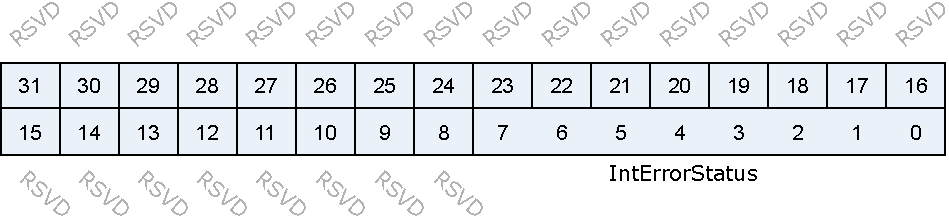
\includegraphics{dma_DMA_IntErrorStatus.pdf}
\end{figure}

\regdes{31:8&RSVD& & & \\\hline
7:0&IntErrorStatus&r&0&Interrupt error status\\\hline

}
\subsection{DMA\_IntErrClr}
\label{dma-DMA-IntErrClr}
Address:0x2000c010
 \begin{figure}[H]
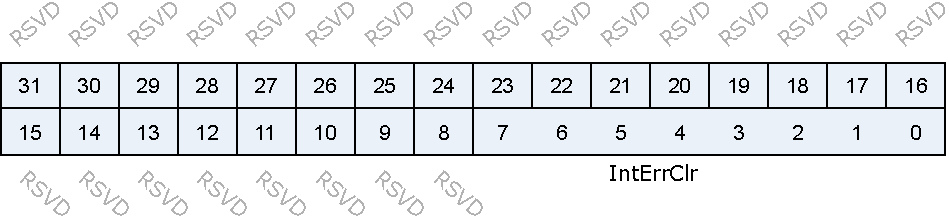
\includegraphics{dma_DMA_IntErrClr.pdf}
\end{figure}

\regdes{31:8&RSVD& & & \\\hline
7:0&IntErrClr&w&0&Interrupt error clear\\\hline

}
\subsection{DMA\_RawIntTCStatus}
\label{dma-DMA-RawIntTCStatus}
Address:0x2000c014
 \begin{figure}[H]
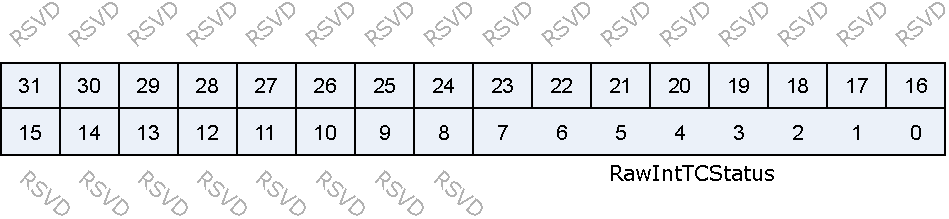
\includegraphics{dma_DMA_RawIntTCStatus.pdf}
\end{figure}

\regdes{31:8&RSVD& & & \\\hline
7:0&RawIntTCStatus&r&0&Status of the terminal count interrupt prior to masking\\\hline

}
\subsection{DMA\_RawIntErrorStatus}
\label{dma-DMA-RawIntErrorStatus}
Address:0x2000c018
 \begin{figure}[H]
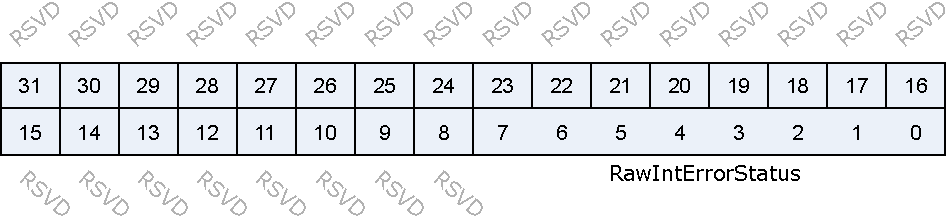
\includegraphics{dma_DMA_RawIntErrorStatus.pdf}
\end{figure}

\regdes{31:8&RSVD& & & \\\hline
7:0&RawIntErrorStatus&r&0&Status of the error interrupt prior to masking\\\hline

}
\subsection{DMA\_EnbldChns}
\label{dma-DMA-EnbldChns}
Address:0x2000c01c
 \begin{figure}[H]
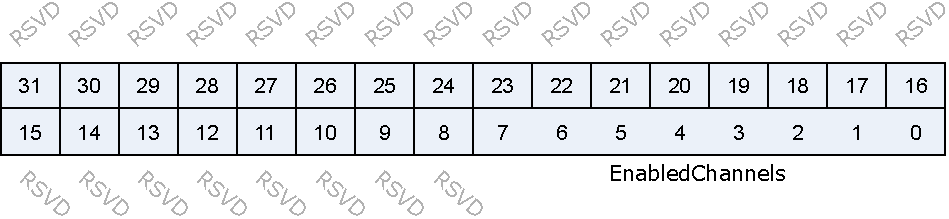
\includegraphics{dma_DMA_EnbldChns.pdf}
\end{figure}

\regdes{31:8&RSVD& & & \\\hline
7:0&EnabledChannels&r&0&Channel enable status\\\hline

}
\subsection{DMA\_SoftBReq}
\label{dma-DMA-SoftBReq}
Address:0x2000c020
 \begin{figure}[H]
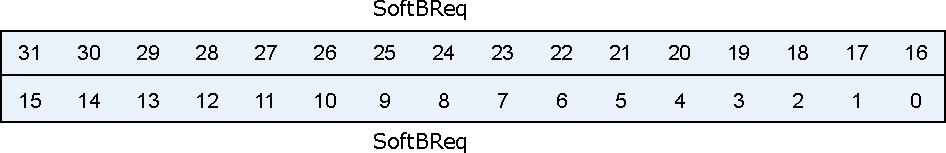
\includegraphics{dma_DMA_SoftBReq.pdf}
\end{figure}

\regdes{31:0&SoftBReq&r/w&0&Software burst request\\\hline

}
\subsection{DMA\_SoftSReq}
\label{dma-DMA-SoftSReq}
Address:0x2000c024
 \begin{figure}[H]
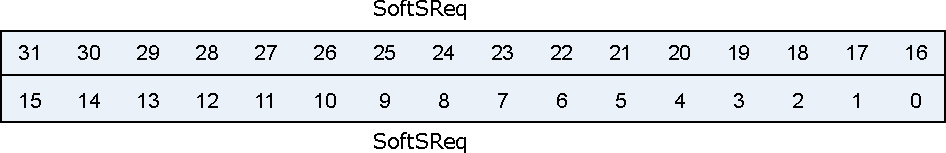
\includegraphics{dma_DMA_SoftSReq.pdf}
\end{figure}

\regdes{31:0&SoftSReq&r/w&0&Software single request\\\hline

}
\subsection{DMA\_SoftLBReq}
\label{dma-DMA-SoftLBReq}
Address:0x2000c028
 \begin{figure}[H]
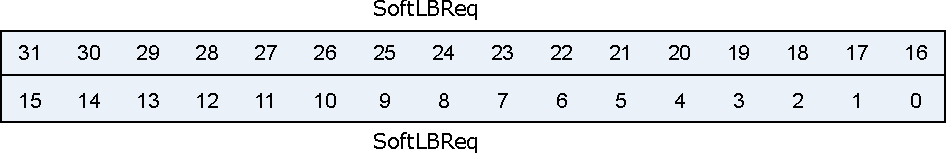
\includegraphics{dma_DMA_SoftLBReq.pdf}
\end{figure}

\regdes{31:0&SoftLBReq&r/w&0&Software last burst request\\\hline

}
\subsection{DMA\_SoftLSReq}
\label{dma-DMA-SoftLSReq}
Address:0x2000c02c
 \begin{figure}[H]
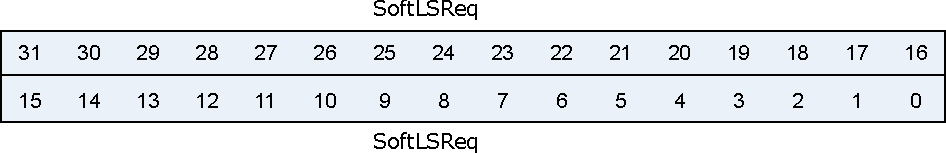
\includegraphics{dma_DMA_SoftLSReq.pdf}
\end{figure}

\regdes{31:0&SoftLSReq&r/w&0&Software last single request\\\hline

}
\subsection{DMA\_Config}
\label{dma-DMA-Config}
Address:0x2000c030
 \begin{figure}[H]
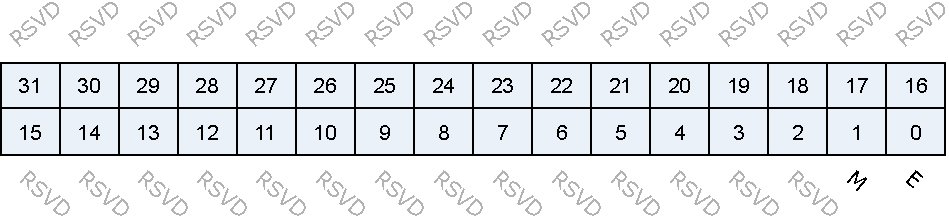
\includegraphics{dma_DMA_Config.pdf}
\end{figure}

\regdes{31:2&RSVD& & & \\\hline
1&M&r/w&0&AHB Master endianness configuration: 0 = little-endian, 1 = big-endian\\\hline
0&E&r/w&0&SMDMA Enable.\\\hline

}
\subsection{DMA\_Sync}
\label{dma-DMA-Sync}
Address:0x2000c034
 \begin{figure}[H]
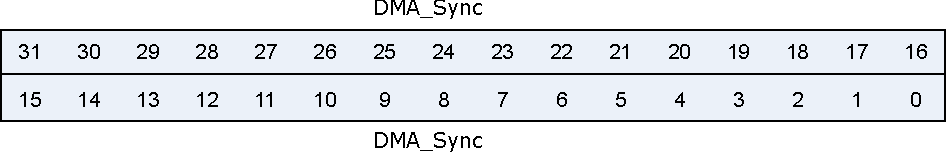
\includegraphics{dma_DMA_Sync.pdf}
\end{figure}

\regdes{31:0&DMA\_Sync&r/w&0&DMA synchronization logic for DMA request signals: 0 = enable, 1 = disable\\\hline

}
\subsection{DMA\_C0SrcAddr}
\label{dma-DMA-C0SrcAddr}
Address:0x2000c100
 \begin{figure}[H]
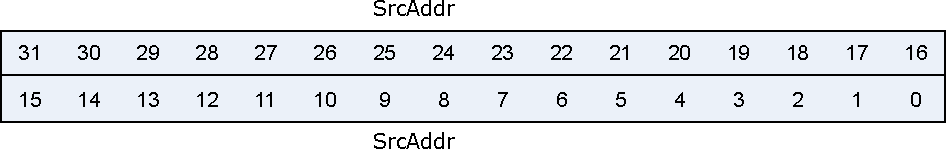
\includegraphics{dma_DMA_C0SrcAddr.pdf}
\end{figure}

\regdes{31:0&SrcAddr&r/w&0&DMA source address\\\hline

}
\subsection{DMA\_C0DstAddr}
\label{dma-DMA-C0DstAddr}
Address:0x2000c104
 \begin{figure}[H]
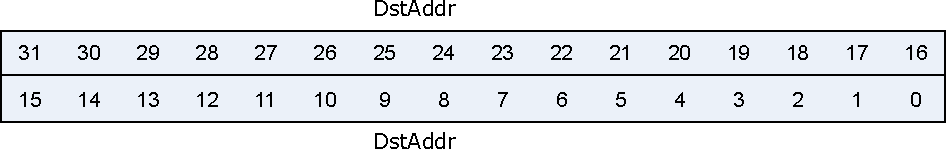
\includegraphics{dma_DMA_C0DstAddr.pdf}
\end{figure}

\regdes{31:0&DstAddr&r/w&0&DMA Destination address\\\hline

}
\subsection{DMA\_C0LLI}
\label{dma-DMA-C0LLI}
Address:0x2000c108
 \begin{figure}[H]
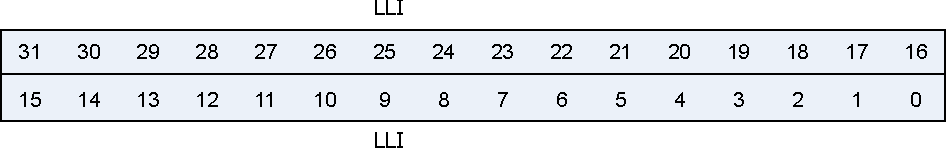
\includegraphics{dma_DMA_C0LLI.pdf}
\end{figure}

\regdes{31:0&LLI&r/w&0&First linked list item. Bits [1:0] must be 0.\\\hline

}
\subsection{DMA\_C0Control}
\label{dma-DMA-C0Control}
Address:0x2000c10c
 \begin{figure}[H]
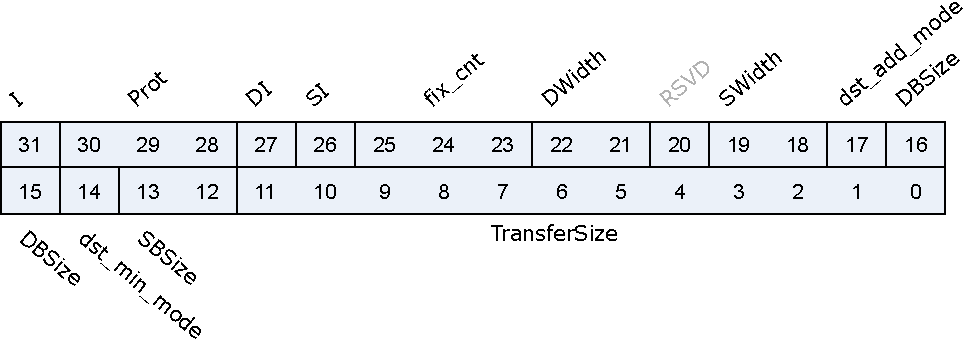
\includegraphics{dma_DMA_C0Control.pdf}
\end{figure}

\regdes{31&I&r/w&0&Terminal count interrupt enable bit. It controls whether the current LLI is expected to trigger the terminal count interrupt.\\\hline
30:28&Prot&r/w&0&No use for currently\\\hline
27&DI&r/w&1&Destination increment. When set, the Destination address is incremented after each transfer.\\\hline
26&SI&r/w&1&Source increment. When set, the source address is incremented after each transfer.\\\hline
25:23&fix\_cnt&r/w&3'd0&Only effect when dst\_min\_mode = 1 \par Destination transfer cnt = (total src byte cnt - (fix\_cnt<<DWidth))<<DWidth
\\\hline
22:21&DWidth&r/w&2'b10&Destination transfer width:  \par 2'b00 : byte \par 2'b01 : half-word \par 2'b10 : word \par 2'b11 : double-word
\\\hline
20&RSVD& & & \\\hline
19:18&SWidth&r/w&2'b10&Source transfer width \par 2'b00 : byte \par 2'b01 : half-word \par 2'b10 : word \par 2'b11 : double-word
\\\hline
17&dst\_add\_mode&r/w&1'b0&Add mode : issue remain destination traffic\\\hline
16:15&DBSize&r/w&2'b01&Destination burst size \par 2'b00 : INCR1 \par 2'b01 : INCR4 \par 2'b10 : INCR8 \par 2'b11 : INCR16 \par Note : SBSize*Swidth should <= CH FIFO Size
\\\hline
14&dst\_min\_mode&r/w&1'b0&Minus mode : Not issue all destination traffic\\\hline
13:12&SBSize&r/w&2'b01&Source burst size:  \par 2'b00 : INCR1 \par 2'b01 : INCR4 \par 2'b10 : INCR8 \par 2'b11 : INCR16 \par Note : SBSize*Swidth should <= CH FIFO Size
\\\hline
11:0&TransferSize&r/w&0&Transfer size: 0~4095. Number of data transfers left to complete when the SMDMA is the flow controller.\\\hline

}
\subsection{DMA\_C0Config}
\label{dma-DMA-C0Config}
Address:0x2000c110
 \begin{figure}[H]
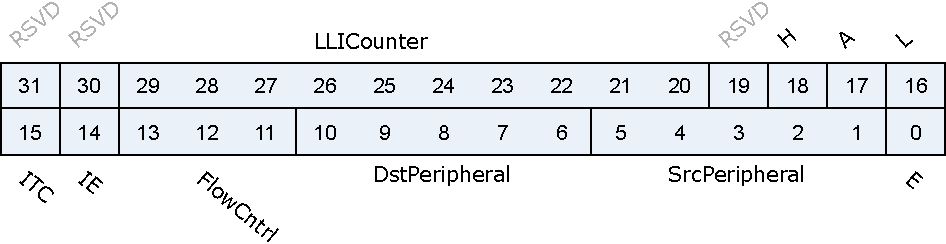
\includegraphics{dma_DMA_C0Config.pdf}
\end{figure}

\regdes{31:30&RSVD& & & \\\hline
29:20&LLICounter&r&0&LLI counter. Increased 1 each LLI run. Cleared 0 when config Control.\\\hline
19&RSVD& & & \\\hline
18&H&r/w&0&Halt: 0 = enable DMA requests, 1 = ignore subsequent source DMA requests.\\\hline
17&A&r&0&Active: 0 = no data in FIFO of the channel, 1 = FIFO of the channel has data.\\\hline
16&L&r/w&0&Lock.\\\hline
15&ITC&r/w&0&Terminal count interrupt mask.\\\hline
14&IE&r/w&0&Interrupt error mask.\\\hline
13:11&FlowCntrl&r/w&0&000: Memory-to-memory (DMA) \par 001: Memory-to-peripheral (DMA) \par 010: Peripheral-to-memory (DMA) \par 011: Source peripheral-to-Destination peripheral (DMA) \par 100: Source peripheral-to-Destination peripheral (Destination peripheral) \par 101: Memory-to-peripheral (peripheral) \par 110: Peripheral-to-memory (peripheral) \par 111: Source peripheral-to-Destination peripheral (Source peripheral)
\\\hline
10:6&DstPeripheral&r/w&0&Destination peripheral.\\\hline
5:1&SrcPeripheral&r/w&0&Source peripheral.\\\hline
0&E&r/w&0&Channel enable.\\\hline

}
\subsection{DMA\_C0RSVD}
\label{dma-DMA-C0RSVD}
Address:0x2000c11c
 \begin{figure}[H]
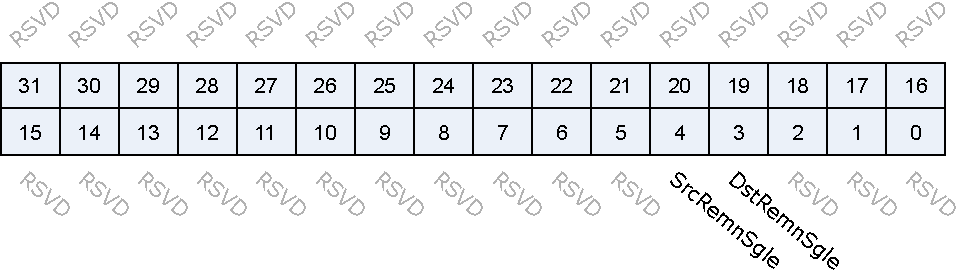
\includegraphics{dma_DMA_C0RSVD.pdf}
\end{figure}

\regdes{31:5&RSVD& & & \\\hline
4&SrcRemnSgle&r/w&0&Source remain single issue mode\\\hline
3&DstRemnSgle&r/w&0&Destination remain single issue mode\\\hline
2:0&RSVD& & & \\\hline

}
\subsection{DMA\_C1SrcAddr}
\label{dma-DMA-C1SrcAddr}
Address:0x2000c200
 \begin{figure}[H]
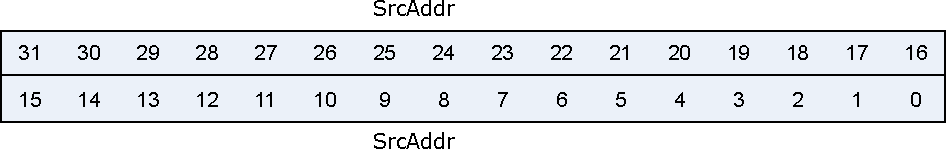
\includegraphics{dma_DMA_C1SrcAddr.pdf}
\end{figure}

\regdes{31:0&SrcAddr&r/w&0&\\\hline

}
\subsection{DMA\_C1DstAddr}
\label{dma-DMA-C1DstAddr}
Address:0x2000c204
 \begin{figure}[H]
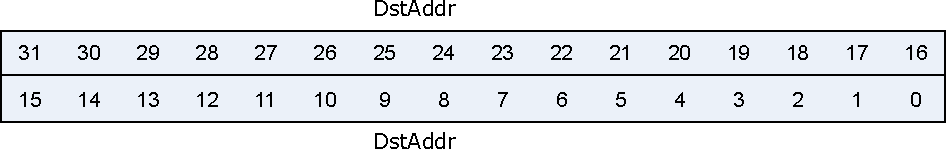
\includegraphics{dma_DMA_C1DstAddr.pdf}
\end{figure}

\regdes{31:0&DstAddr&r/w&0&\\\hline

}
\subsection{DMA\_C1LLI}
\label{dma-DMA-C1LLI}
Address:0x2000c208
 \begin{figure}[H]
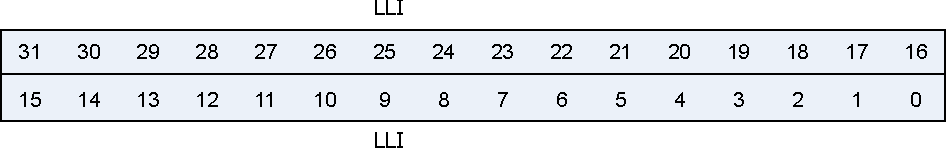
\includegraphics{dma_DMA_C1LLI.pdf}
\end{figure}

\regdes{31:0&LLI&r/w&0&\\\hline

}
\subsection{DMA\_C1Control}
\label{dma-DMA-C1Control}
Address:0x2000c20c
 \begin{figure}[H]
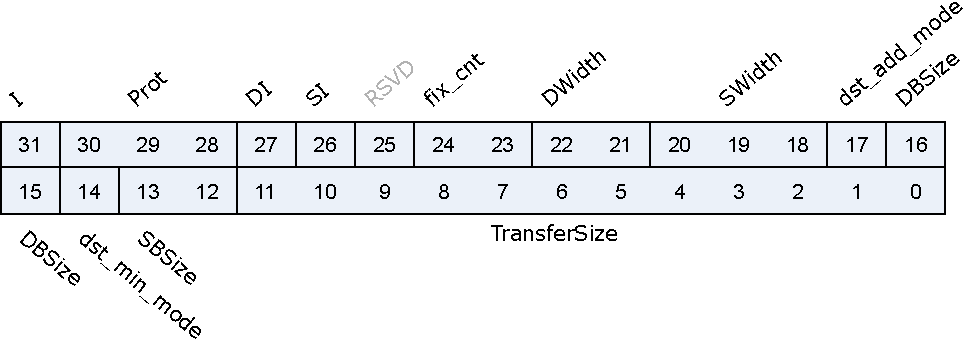
\includegraphics{dma_DMA_C1Control.pdf}
\end{figure}

\regdes{31&I&r/w&0&Terminal count interrupt enable bit. It controls whether the current LLI is expected to trigger the terminal count interrupt.\\\hline
30:28&Prot&r/w&0&No use for currently\\\hline
27&DI&r/w&1&Destination increment. When set, the Destination address is incremented after each transfer.\\\hline
26&SI&r/w&1&Source increment. When set, the source address is incremented after each transfer.\\\hline
25:23&fix\_cnt&r/w&3'd0&Only effect when dst\_min\_mode = 1 \par Destination transfer cnt = (total src byte cnt - (fix\_cnt<<DWidth))<<DWidth
\\\hline
22:21&DWidth&r/w&2'b10&Destination transfer width:  \par 2'b00 : byte \par 2'b01 : half-word \par 2'b10 : word \par 2'b11 : double-word
\\\hline
20&RSVD& & & \\\hline
19:18&SWidth&r/w&2'b10&Source transfer width \par 2'b00 : byte \par 2'b01 : half-word \par 2'b10 : word \par 2'b11 : double-word
\\\hline
17&dst\_add\_mode&r/w&1'b0&Add mode : issue remain destination traffic\\\hline
16:15&DBSize&r/w&2'b01&Destination burst size \par 2'b00 : INCR1 \par 2'b01 : INCR4 \par 2'b10 : INCR8 \par 2'b11 : INCR16 \par Note : SBSize*Swidth should <= CH FIFO Size
\\\hline
14&dst\_min\_mode&r/w&1'b0&Minus mode : Not issue all destination traffic\\\hline
13:12&SBSize&r/w&2'b01&Source burst size:  \par 2'b00 : INCR1 \par 2'b01 : INCR4 \par 2'b10 : INCR8 \par 2'b11 : INCR16 \par Note : SBSize*Swidth should <= CH FIFO Size
\\\hline
11:0&TransferSize&r/w&0&Transfer size: 0~4095. Number of data transfers left to complete when the SMDMA is the flow controller.\\\hline

}
\subsection{DMA\_C1Config}
\label{dma-DMA-C1Config}
Address:0x2000c210
 \begin{figure}[H]
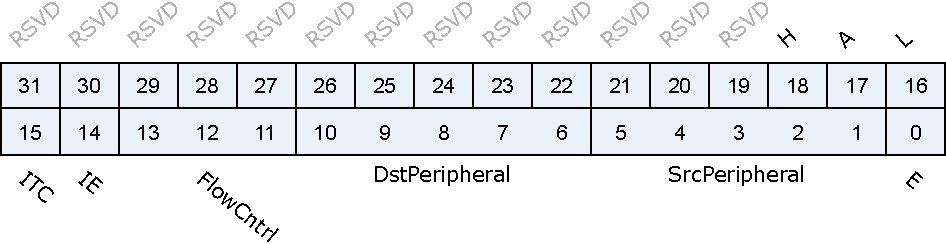
\includegraphics{dma_DMA_C1Config.pdf}
\end{figure}

\regdes{31:19&RSVD& & & \\\hline
18&H&r/w&0&\\\hline
17&A&r&0&\\\hline
16&L&r/w&0&\\\hline
15&ITC&r/w&0&\\\hline
14&IE&r/w&0&\\\hline
13:11&FlowCntrl&r/w&0&\\\hline
10:6&DstPeripheral&r/w&0&\\\hline
5:1&SrcPeripheral&r/w&0&\\\hline
0&E&r/w&0&\\\hline

}
\subsection{DMA\_C1RSVD}
\label{dma-DMA-C1RSVD}
Address:0x2000c21c
 \begin{figure}[H]
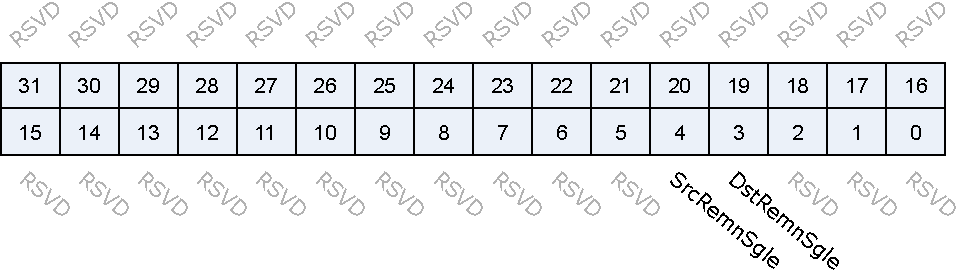
\includegraphics{dma_DMA_C1RSVD.pdf}
\end{figure}

\regdes{31:5&RSVD& & & \\\hline
4&SrcRemnSgle&r/w&0&Source remain single issue mode\\\hline
3&DstRemnSgle&r/w&0&Destination remain single issue mode\\\hline
2:0&RSVD& & & \\\hline

}
\subsection{DMA\_C2SrcAddr}
\label{dma-DMA-C2SrcAddr}
Address:0x2000c300
 \begin{figure}[H]
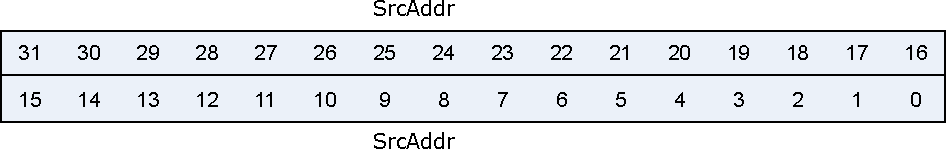
\includegraphics{dma_DMA_C2SrcAddr.pdf}
\end{figure}

\regdes{31:0&SrcAddr&r/w&0&\\\hline

}
\subsection{DMA\_C2DstAddr}
\label{dma-DMA-C2DstAddr}
Address:0x2000c304
 \begin{figure}[H]
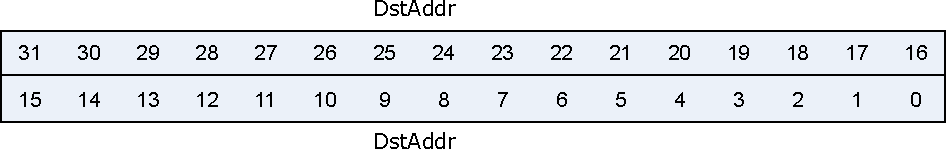
\includegraphics{dma_DMA_C2DstAddr.pdf}
\end{figure}

\regdes{31:0&DstAddr&r/w&0&\\\hline

}
\subsection{DMA\_C2LLI}
\label{dma-DMA-C2LLI}
Address:0x2000c308
 \begin{figure}[H]
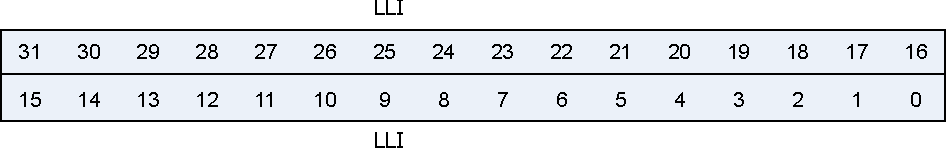
\includegraphics{dma_DMA_C2LLI.pdf}
\end{figure}

\regdes{31:0&LLI&r/w&0&\\\hline

}
\subsection{DMA\_C2Control}
\label{dma-DMA-C2Control}
Address:0x2000c30c
 \begin{figure}[H]
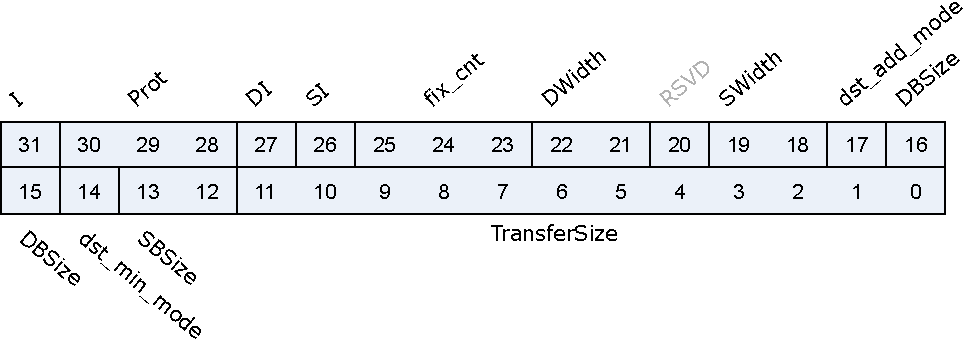
\includegraphics{dma_DMA_C2Control.pdf}
\end{figure}

\regdes{31&I&r/w&0&Terminal count interrupt enable bit. It controls whether the current LLI is expected to trigger the terminal count interrupt.\\\hline
30:28&Prot&r/w&0&No use for currently\\\hline
27&DI&r/w&1&Destination increment. When set, the Destination address is incremented after each transfer.\\\hline
26&SI&r/w&1&Source increment. When set, the source address is incremented after each transfer.\\\hline
25:23&fix\_cnt&r/w&3'd0&Only effect when dst\_min\_mode = 1 \par Destination transfer cnt = (total src byte cnt - (fix\_cnt<<DWidth))<<DWidth
\\\hline
22:21&DWidth&r/w&2'b10&Destination transfer width:  \par 2'b00 : byte \par 2'b01 : half-word \par 2'b10 : word \par 2'b11 : double-word
\\\hline
20&RSVD& & & \\\hline
19:18&SWidth&r/w&2'b10&Source transfer width \par 2'b00 : byte \par 2'b01 : half-word \par 2'b10 : word \par 2'b11 : double-word
\\\hline
17&dst\_add\_mode&r/w&1'b0&Add mode : issue remain destination traffic\\\hline
16:15&DBSize&r/w&2'b01&Destination burst size \par 2'b00 : INCR1 \par 2'b01 : INCR4 \par 2'b10 : INCR8 \par 2'b11 : INCR16 \par Note : SBSize*Swidth should <= CH FIFO Size
\\\hline
14&dst\_min\_mode&r/w&1'b0&Minus mode : Not issue all destination traffic\\\hline
13:12&SBSize&r/w&2'b01&Source burst size:  \par 2'b00 : INCR1 \par 2'b01 : INCR4 \par 2'b10 : INCR8 \par 2'b11 : INCR16 \par Note : SBSize*Swidth should <= CH FIFO Size
\\\hline
11:0&TransferSize&r/w&0&Transfer size: 0~4095. Number of data transfers left to complete when the SMDMA is the flow controller.\\\hline

}
\subsection{DMA\_C2Config}
\label{dma-DMA-C2Config}
Address:0x2000c310
 \begin{figure}[H]
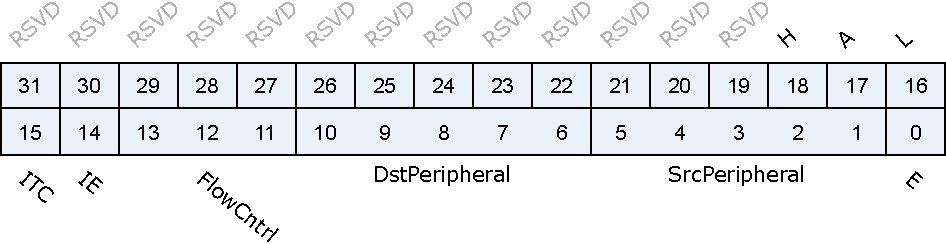
\includegraphics{dma_DMA_C2Config.pdf}
\end{figure}

\regdes{31:19&RSVD& & & \\\hline
18&H&r/w&0&\\\hline
17&A&r&0&\\\hline
16&L&r/w&0&\\\hline
15&ITC&r/w&0&\\\hline
14&IE&r/w&0&\\\hline
13:11&FlowCntrl&r/w&0&\\\hline
10:6&DstPeripheral&r/w&0&\\\hline
5:1&SrcPeripheral&r/w&0&\\\hline
0&E&r/w&0&\\\hline

}
\subsection{DMA\_C2RSVD}
\label{dma-DMA-C2RSVD}
Address:0x2000c31c
 \begin{figure}[H]
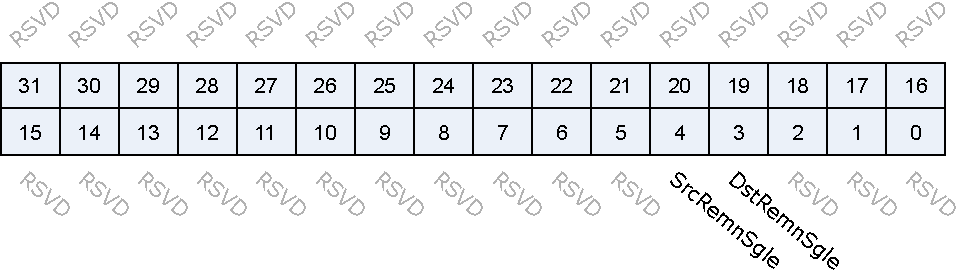
\includegraphics{dma_DMA_C2RSVD.pdf}
\end{figure}

\regdes{31:5&RSVD& & & \\\hline
4&SrcRemnSgle&r/w&0&Source remain single issue mode\\\hline
3&DstRemnSgle&r/w&0&Destination remain single issue mode\\\hline
2:0&RSVD& & & \\\hline

}
\subsection{DMA\_C3SrcAddr}
\label{dma-DMA-C3SrcAddr}
Address:0x2000c400
 \begin{figure}[H]
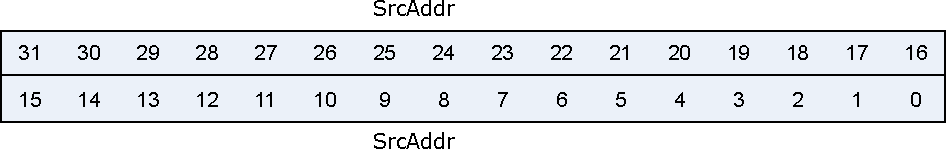
\includegraphics{dma_DMA_C3SrcAddr.pdf}
\end{figure}

\regdes{31:0&SrcAddr&r/w&0&\\\hline

}
\subsection{DMA\_C3DstAddr}
\label{dma-DMA-C3DstAddr}
Address:0x2000c404
 \begin{figure}[H]
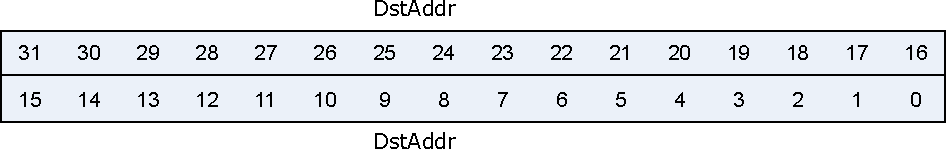
\includegraphics{dma_DMA_C3DstAddr.pdf}
\end{figure}

\regdes{31:0&DstAddr&r/w&0&\\\hline

}
\subsection{DMA\_C3LLI}
\label{dma-DMA-C3LLI}
Address:0x2000c408
 \begin{figure}[H]
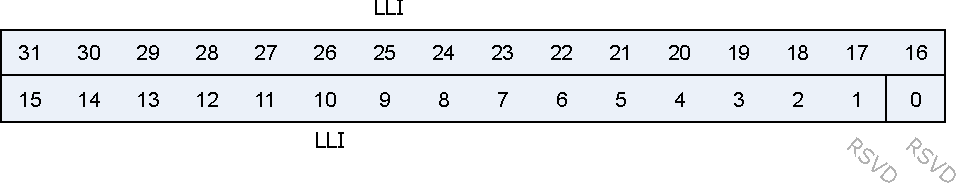
\includegraphics{dma_DMA_C3LLI.pdf}
\end{figure}

\regdes{31:0&LLI&r/w&0&\\\hline

}
\subsection{DMA\_C3Control}
\label{dma-DMA-C3Control}
Address:0x2000c40c
 \begin{figure}[H]
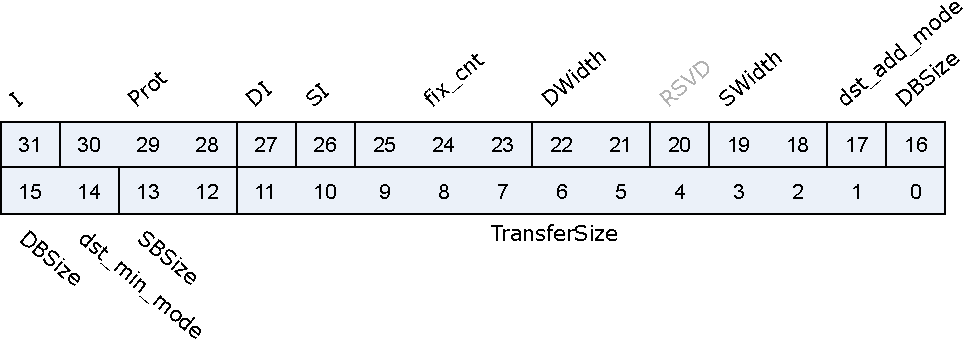
\includegraphics{dma_DMA_C3Control.pdf}
\end{figure}

\regdes{31&I&r/w&0&Terminal count interrupt enable bit. It controls whether the current LLI is expected to trigger the terminal count interrupt.\\\hline
30:28&Prot&r/w&0&No use for currently\\\hline
27&DI&r/w&1&Destination increment. When set, the Destination address is incremented after each transfer.\\\hline
26&SI&r/w&1&Source increment. When set, the source address is incremented after each transfer.\\\hline
25:23&fix\_cnt&r/w&3'd0&Only effect when dst\_min\_mode = 1 \par Destination transfer cnt = (total src byte cnt - (fix\_cnt<<DWidth))<<DWidth
\\\hline
22:21&DWidth&r/w&2'b10&Destination transfer width:  \par 2'b00 : byte \par 2'b01 : half-word \par 2'b10 : word \par 2'b11 : double-word
\\\hline
20&RSVD& & & \\\hline
19:18&SWidth&r/w&2'b10&Source transfer width \par 2'b00 : byte \par 2'b01 : half-word \par 2'b10 : word \par 2'b11 : double-word
\\\hline
17&dst\_add\_mode&r/w&1'b0&Add mode : issue remain destination traffic\\\hline
16:15&DBSize&r/w&2'b01&Destination burst size \par 2'b00 : INCR1 \par 2'b01 : INCR4 \par 2'b10 : INCR8 \par 2'b11 : INCR16 \par Note : SBSize*Swidth should <= CH FIFO Size
\\\hline
14&dst\_min\_mode&r/w&1'b0&Minus mode : Not issue all destination traffic\\\hline
13:12&SBSize&r/w&2'b01&Source burst size:  \par 2'b00 : INCR1 \par 2'b01 : INCR4 \par 2'b10 : INCR8 \par 2'b11 : INCR16 \par Note : SBSize*Swidth should <= CH FIFO Size
\\\hline
11:0&TransferSize&r/w&0&Transfer size: 0~4095. Number of data transfers left to complete when the SMDMA is the flow controller.\\\hline

}
\subsection{DMA\_C3Config}
\label{dma-DMA-C3Config}
Address:0x2000c310
 \begin{figure}[H]
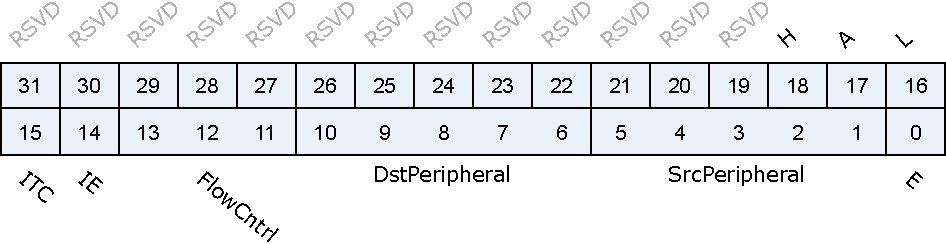
\includegraphics{dma_DMA_C3Config.pdf}
\end{figure}

\regdes{31:19&RSVD& & & \\\hline
18&H&r/w&0&\\\hline
17&A&r&0&\\\hline
16&L&r/w&0&\\\hline
15&ITC&r/w&0&\\\hline
14&IE&r/w&0&\\\hline
13:11&FlowCntrl&r/w&0&\\\hline
10:6&DstPeripheral&r/w&0&\\\hline
5:1&SrcPeripheral&r/w&0&\\\hline
0&E&r/w&0&\\\hline

}
\subsection{DMA\_C3RSVD}
\label{dma-DMA-C3RSVD}
Address:0x2000c31c
 \begin{figure}[H]
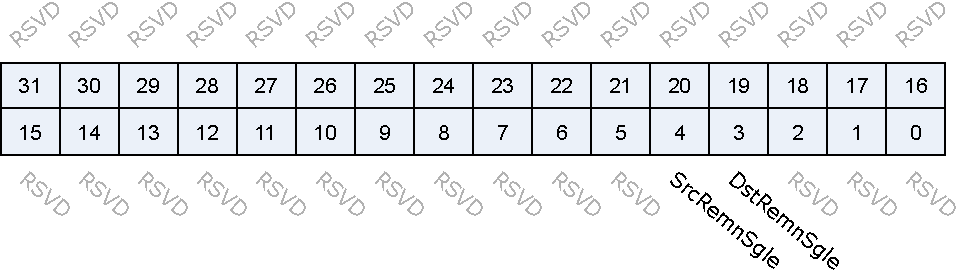
\includegraphics{dma_DMA_C3RSVD.pdf}
\end{figure}

\regdes{31:5&RSVD& & & \\\hline
4&SrcRemnSgle&r/w&0&Source remain single issue mode\\\hline
3&DstRemnSgle&r/w&0&Destination remain single issue mode\\\hline
2:0&RSVD& & & \\\hline

}
\subsection{DMA\_C4SrcAddr}
\label{dma-DMA-C4SrcAddr}
Address:0x2000c500
 \begin{figure}[H]
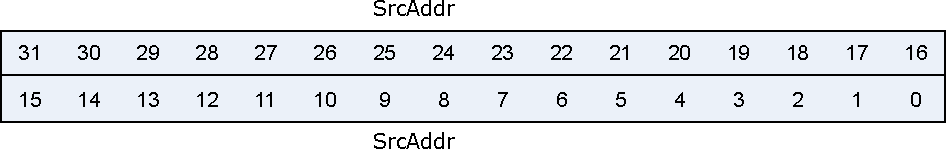
\includegraphics{dma_DMA_C4SrcAddr.pdf}
\end{figure}

\regdes{31:0&SrcAddr&r/w&0&\\\hline

}
\subsection{DMA\_C4DstAddr}
\label{dma-DMA-C4DstAddr}
Address:0x2000c504
 \begin{figure}[H]
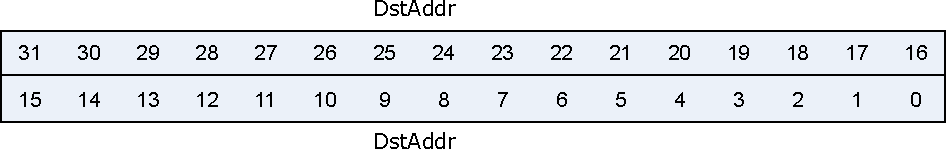
\includegraphics{dma_DMA_C4DstAddr.pdf}
\end{figure}

\regdes{31:0&DstAddr&r/w&0&\\\hline

}
\subsection{DMA\_C4LLI}
\label{dma-DMA-C4LLI}
Address:0x2000c508
 \begin{figure}[H]
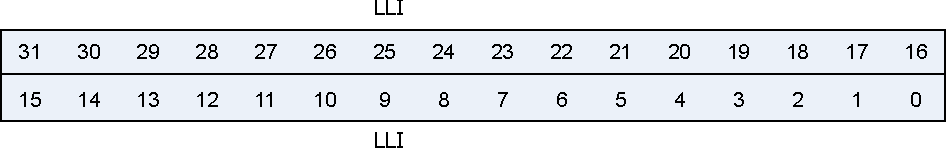
\includegraphics{dma_DMA_C4LLI.pdf}
\end{figure}

\regdes{31:0&LLI&r/w&0&\\\hline

}
\subsection{DMA\_C4Control}
\label{dma-DMA-C4Control}
Address:0x2000c50c
 \begin{figure}[H]
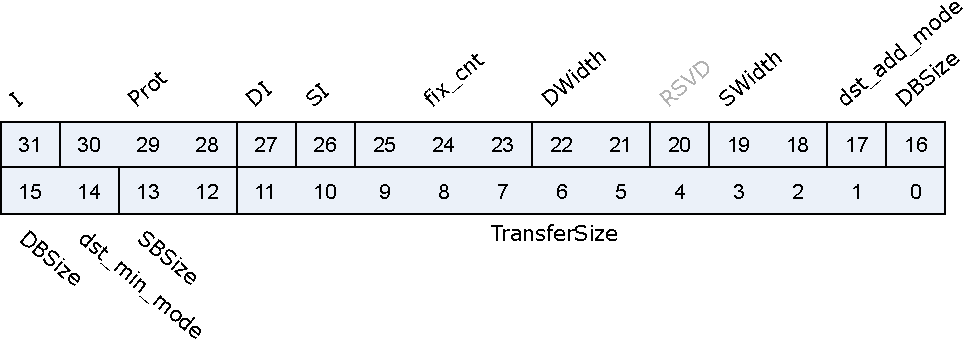
\includegraphics{dma_DMA_C4Control.pdf}
\end{figure}

\regdes{31&I&r/w&0&Terminal count interrupt enable bit. It controls whether the current LLI is expected to trigger the terminal count interrupt.\\\hline
30:28&Prot&r/w&0&No use for currently\\\hline
27&DI&r/w&1&Destination increment. When set, the Destination address is incremented after each transfer.\\\hline
26&SI&r/w&1&Source increment. When set, the source address is incremented after each transfer.\\\hline
25:23&fix\_cnt&r/w&3'd0&Only effect when dst\_min\_mode = 1 \par Destination transfer cnt = (total src byte cnt - (fix\_cnt<<DWidth))<<DWidth
\\\hline
22:21&DWidth&r/w&2'b10&Destination transfer width:  \par 2'b00 : byte \par 2'b01 : half-word \par 2'b10 : word \par 2'b11 : double-word
\\\hline
20&RSVD& & & \\\hline
19:18&SWidth&r/w&2'b10&Source transfer width \par 2'b00 : byte \par 2'b01 : half-word \par 2'b10 : word \par 2'b11 : double-word
\\\hline
17&dst\_add\_mode&r/w&1'b0&Add mode : issue remain destination traffic\\\hline
16:15&DBSize&r/w&2'b01&Destination burst size \par 2'b00 : INCR1 \par 2'b01 : INCR4 \par 2'b10 : INCR8 \par 2'b11 : INCR16 \par Note : SBSize*Swidth should <= CH FIFO Size
\\\hline
14&dst\_min\_mode&r/w&1'b0&Minus mode : Not issue all destination traffic\\\hline
13:12&SBSize&r/w&2'b01&Source burst size:  \par 2'b00 : INCR1 \par 2'b01 : INCR4 \par 2'b10 : INCR8 \par 2'b11 : INCR16 \par Note : SBSize*Swidth should <= CH FIFO Size
\\\hline
11:0&TransferSize&r/w&0&Transfer size: 0~4095. Number of data transfers left to complete when the SMDMA is the flow controller.\\\hline

}
\subsection{DMA\_C4Config}
\label{dma-DMA-C4Config}
Address:0x2000c510
 \begin{figure}[H]
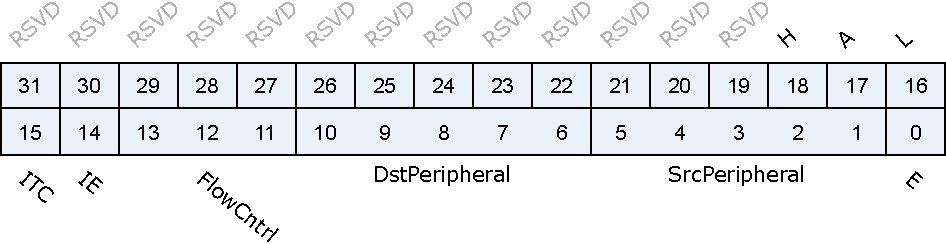
\includegraphics{dma_DMA_C4Config.pdf}
\end{figure}

\regdes{31:19&RSVD& & & \\\hline
18&H&r/w&0&\\\hline
17&A&r&0&\\\hline
16&L&r/w&0&\\\hline
15&ITC&r/w&0&\\\hline
14&IE&r/w&0&\\\hline
13:11&FlowCntrl&r/w&0&\\\hline
10:6&DstPeripheral&r/w&0&\\\hline
5:1&SrcPeripheral&r/w&0&\\\hline
0&E&r/w&0&\\\hline

}
\subsection{DMA\_C4RSVD}
\label{dma-DMA-C4RSVD}
Address:0x2000c51c
 \begin{figure}[H]
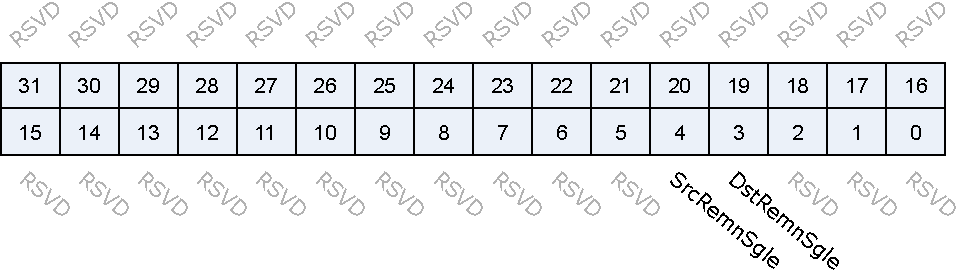
\includegraphics{dma_DMA_C4RSVD.pdf}
\end{figure}

\regdes{31:5&RSVD& & & \\\hline
4&SrcRemnSgle&r/w&0&Source remain single issue mode\\\hline
3&DstRemnSgle&r/w&0&Destination remain single issue mode\\\hline
2:0&RSVD& & & \\\hline

}
\subsection{DMA\_C5SrcAddr}
\label{dma-DMA-C5SrcAddr}
Address:0x2000c600
 \begin{figure}[H]
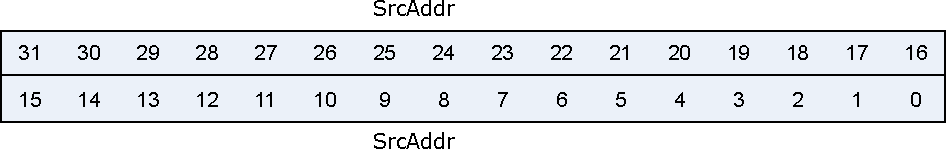
\includegraphics{dma_DMA_C5SrcAddr.pdf}
\end{figure}

\regdes{31:0&SrcAddr&r/w&0&\\\hline

}
\subsection{DMA\_C5DstAddr}
\label{dma-DMA-C5DstAddr}
Address:0x2000c604
 \begin{figure}[H]
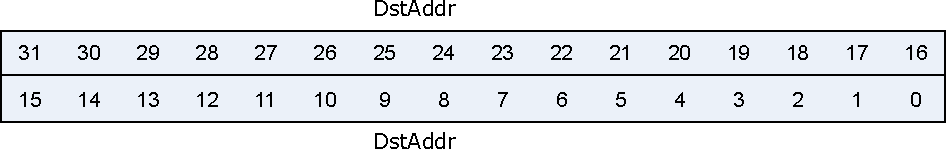
\includegraphics{dma_DMA_C5DstAddr.pdf}
\end{figure}

\regdes{31:0&DstAddr&r/w&0&\\\hline

}
\subsection{DMA\_C5LLI}
\label{dma-DMA-C5LLI}
Address:0x2000c608
 \begin{figure}[H]
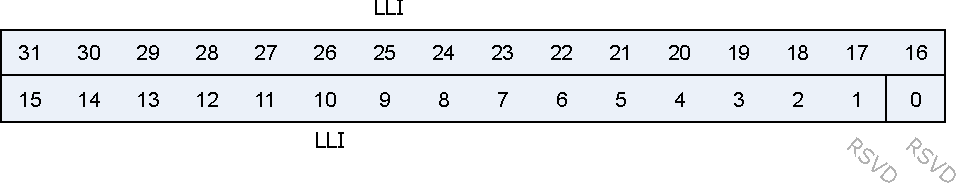
\includegraphics{dma_DMA_C5LLI.pdf}
\end{figure}

\regdes{31:0&LLI&r/w&0&\\\hline

}
\subsection{DMA\_C5Control}
\label{dma-DMA-C5Control}
Address:0x2000c60c
 \begin{figure}[H]
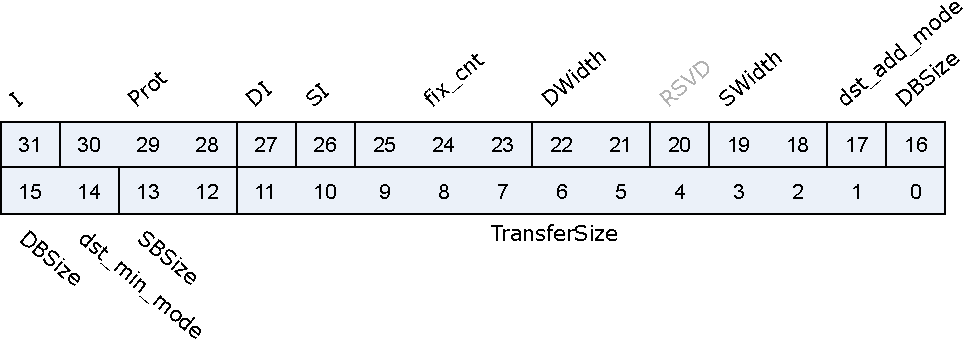
\includegraphics{dma_DMA_C5Control.pdf}
\end{figure}

\regdes{31&I&r/w&0&Terminal count interrupt enable bit. It controls whether the current LLI is expected to trigger the terminal count interrupt.\\\hline
30:28&Prot&r/w&0&No use for currently\\\hline
27&DI&r/w&1&Destination increment. When set, the Destination address is incremented after each transfer.\\\hline
26&SI&r/w&1&Source increment. When set, the source address is incremented after each transfer.\\\hline
25:23&fix\_cnt&r/w&3'd0&Only effect when dst\_min\_mode = 1 \par Destination transfer cnt = (total src byte cnt - (fix\_cnt<<DWidth))<<DWidth
\\\hline
22:21&DWidth&r/w&2'b10&Destination transfer width:  \par 2'b00 : byte \par 2'b01 : half-word \par 2'b10 : word \par 2'b11 : double-word
\\\hline
20&RSVD& & & \\\hline
19:18&SWidth&r/w&2'b10&Source transfer width \par 2'b00 : byte \par 2'b01 : half-word \par 2'b10 : word \par 2'b11 : double-word
\\\hline
17&dst\_add\_mode&r/w&1'b0&Add mode : issue remain destination traffic\\\hline
16:15&DBSize&r/w&2'b01&Destination burst size \par 2'b00 : INCR1 \par 2'b01 : INCR4 \par 2'b10 : INCR8 \par 2'b11 : INCR16 \par Note : SBSize*Swidth should <= CH FIFO Size
\\\hline
14&dst\_min\_mode&r/w&1'b0&Minus mode : Not issue all destination traffic\\\hline
13:12&SBSize&r/w&2'b01&Source burst size:  \par 2'b00 : INCR1 \par 2'b01 : INCR4 \par 2'b10 : INCR8 \par 2'b11 : INCR16 \par Note : SBSize*Swidth should <= CH FIFO Size
\\\hline
11:0&TransferSize&r/w&0&Transfer size: 0~4095. Number of data transfers left to complete when the SMDMA is the flow controller.\\\hline

}
\subsection{DMA\_C5Config}
\label{dma-DMA-C5Config}
Address:0x2000c610
 \begin{figure}[H]
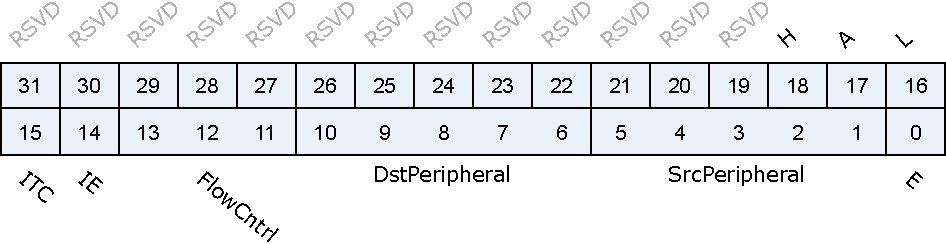
\includegraphics{dma_DMA_C5Config.pdf}
\end{figure}

\regdes{31:19&RSVD& & & \\\hline
18&H&r/w&0&\\\hline
17&A&r&0&\\\hline
16&L&r/w&0&\\\hline
15&ITC&r/w&0&\\\hline
14&IE&r/w&0&\\\hline
13:11&FlowCntrl&r/w&0&\\\hline
10:6&DstPeripheral&r/w&0&\\\hline
5:1&SrcPeripheral&r/w&0&\\\hline
0&E&r/w&0&\\\hline

}
\subsection{DMA\_C5RSVD}
\label{dma-DMA-C5RSVD}
Address:0x2000c61c
 \begin{figure}[H]
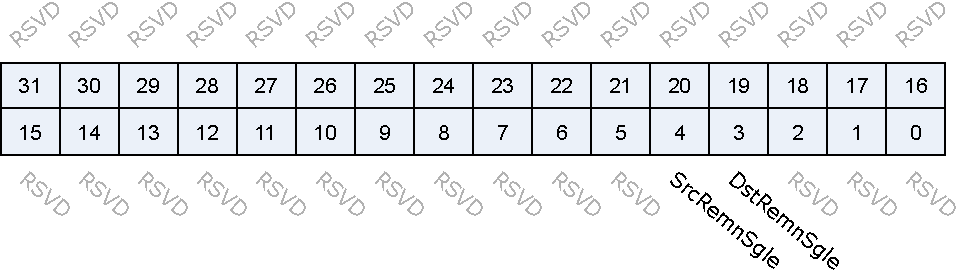
\includegraphics{dma_DMA_C5RSVD.pdf}
\end{figure}

\regdes{31:5&RSVD& & & \\\hline
4&SrcRemnSgle&r/w&0&Source remain single issue mode\\\hline
3&DstRemnSgle&r/w&0&Destination remain single issue mode\\\hline
2:0&RSVD& & & \\\hline

}
\subsection{DMA\_C6SrcAddr}
\label{dma-DMA-C6SrcAddr}
Address:0x2000c700
 \begin{figure}[H]
\includegraphics{dma_DMA_C6SrcAddr.pdf}
\end{figure}

\regdes{31:0&SrcAddr&r/w&0&\\\hline

}
\subsection{DMA\_C6DstAddr}
\label{dma-DMA-C6DstAddr}
Address:0x2000c704
 \begin{figure}[H]
\includegraphics{dma_DMA_C6DstAddr.pdf}
\end{figure}

\regdes{31:0&DstAddr&r/w&0&\\\hline

}
\subsection{DMA\_C6LLI}
\label{dma-DMA-C6LLI}
Address:0x2000c708
 \begin{figure}[H]
\includegraphics{dma_DMA_C6LLI.pdf}
\end{figure}

\regdes{31:0&LLI&r/w&0&\\\hline

}
\subsection{DMA\_C6Control}
\label{dma-DMA-C6Control}
Address:0x2000c70c
 \begin{figure}[H]
\includegraphics{dma_DMA_C6Control.pdf}
\end{figure}

\regdes{31&I&r/w&0&Terminal count interrupt enable bit. It controls whether the current LLI is expected to trigger the terminal count interrupt.\\\hline
30:28&Prot&r/w&0&No use for currently\\\hline
27&DI&r/w&1&Destination increment. When set, the Destination address is incremented after each transfer.\\\hline
26&SI&r/w&1&Source increment. When set, the source address is incremented after each transfer.\\\hline
25:23&fix\_cnt&r/w&3'd0&Only effect when dst\_min\_mode = 1 \par Destination transfer cnt = (total src byte cnt - (fix\_cnt<<DWidth))<<DWidth
\\\hline
22:21&DWidth&r/w&2'b10&Destination transfer width:  \par 2'b00 : byte \par 2'b01 : half-word \par 2'b10 : word \par 2'b11 : double-word
\\\hline
20&RSVD& & & \\\hline
19:18&SWidth&r/w&2'b10&Source transfer width \par 2'b00 : byte \par 2'b01 : half-word \par 2'b10 : word \par 2'b11 : double-word
\\\hline
17&dst\_add\_mode&r/w&1'b0&Add mode : issue remain destination traffic\\\hline
16:15&DBSize&r/w&2'b01&Destination burst size \par 2'b00 : INCR1 \par 2'b01 : INCR4 \par 2'b10 : INCR8 \par 2'b11 : INCR16 \par Note : SBSize*Swidth should <= CH FIFO Size
\\\hline
14&dst\_min\_mode&r/w&1'b0&Minus mode : Not issue all destination traffic\\\hline
13:12&SBSize&r/w&2'b01&Source burst size:  \par 2'b00 : INCR1 \par 2'b01 : INCR4 \par 2'b10 : INCR8 \par 2'b11 : INCR16 \par Note : SBSize*Swidth should <= CH FIFO Size
\\\hline
11:0&TransferSize&r/w&0&Transfer size: 0~4095. Number of data transfers left to complete when the SMDMA is the flow controller.\\\hline

}
\subsection{DMA\_C6Config}
\label{dma-DMA-C6Config}
Address:0x2000c710
 \begin{figure}[H]
\includegraphics{dma_DMA_C6Config.pdf}
\end{figure}

\regdes{31:19&RSVD& & & \\\hline
18&H&r/w&0&\\\hline
17&A&r&0&\\\hline
16&L&r/w&0&\\\hline
15&ITC&r/w&0&\\\hline
14&IE&r/w&0&\\\hline
13:11&FlowCntrl&r/w&0&\\\hline
10:6&DstPeripheral&r/w&0&\\\hline
5:1&SrcPeripheral&r/w&0&\\\hline
0&E&r/w&0&\\\hline

}
\subsection{DMA\_C6RSVD}
\label{dma-DMA-C6RSVD}
Address:0x2000c71c
 \begin{figure}[H]
\includegraphics{dma_DMA_C6RSVD.pdf}
\end{figure}

\regdes{31:5&RSVD& & & \\\hline
4&SrcRemnSgle&r/w&0&Source remain single issue mode\\\hline
3&DstRemnSgle&r/w&0&Destination remain single issue mode\\\hline
2:0&RSVD& & & \\\hline

}
\subsection{DMA\_C7SrcAddr}
\label{dma-DMA-C7SrcAddr}
Address:0x2000c800
 \begin{figure}[H]
\includegraphics{dma_DMA_C7SrcAddr.pdf}
\end{figure}

\regdes{31:0&SrcAddr&r/w&0&\\\hline

}
\subsection{DMA\_C7DstAddr}
\label{dma-DMA-C7DstAddr}
Address:0x2000c804
 \begin{figure}[H]
\includegraphics{dma_DMA_C7DstAddr.pdf}
\end{figure}

\regdes{31:0&DstAddr&r/w&0&\\\hline

}
\subsection{DMA\_C7LLI}
\label{dma-DMA-C7LLI}
Address:0x2000c808
 \begin{figure}[H]
\includegraphics{dma_DMA_C7LLI.pdf}
\end{figure}

\regdes{31:0&LLI&r/w&0&\\\hline

}
\subsection{DMA\_C7Control}
\label{dma-DMA-C7Control}
Address:0x2000c80c
 \begin{figure}[H]
\includegraphics{dma_DMA_C7Control.pdf}
\end{figure}

\regdes{31&I&r/w&0&Terminal count interrupt enable bit. It controls whether the current LLI is expected to trigger the terminal count interrupt.\\\hline
30:28&Prot&r/w&0&No use for currently\\\hline
27&DI&r/w&1&Destination increment. When set, the Destination address is incremented after each transfer.\\\hline
26&SI&r/w&1&Source increment. When set, the source address is incremented after each transfer.\\\hline
25:23&fix\_cnt&r/w&3'd0&Only effect when dst\_min\_mode = 1 \par Destination transfer cnt = (total src byte cnt - (fix\_cnt<<DWidth))<<DWidth
\\\hline
22:21&DWidth&r/w&2'b10&Destination transfer width:  \par 2'b00 : byte \par 2'b01 : half-word \par 2'b10 : word \par 2'b11 : double-word
\\\hline
20&RSVD& & & \\\hline
19:18&SWidth&r/w&2'b10&Source transfer width \par 2'b00 : byte \par 2'b01 : half-word \par 2'b10 : word \par 2'b11 : double-word
\\\hline
17&dst\_add\_mode&r/w&1'b0&Add mode : issue remain destination traffic\\\hline
16:15&DBSize&r/w&2'b01&Destination burst size \par 2'b00 : INCR1 \par 2'b01 : INCR4 \par 2'b10 : INCR8 \par 2'b11 : INCR16 \par Note : SBSize*Swidth should <= CH FIFO Size
\\\hline
14&dst\_min\_mode&r/w&1'b0&Minus mode : Not issue all destination traffic\\\hline
13:12&SBSize&r/w&2'b01&Source burst size:  \par 2'b00 : INCR1 \par 2'b01 : INCR4 \par 2'b10 : INCR8 \par 2'b11 : INCR16 \par Note : SBSize*Swidth should <= CH FIFO Size
\\\hline
11:0&TransferSize&r/w&0&Transfer size: 0~4095. Number of data transfers left to complete when the SMDMA is the flow controller.\\\hline

}
\subsection{DMA\_C7Config}
\label{dma-DMA-C7Config}
Address:0x2000c810
 \begin{figure}[H]
\includegraphics{dma_DMA_C7Config.pdf}
\end{figure}

\regdes{31:19&RSVD& & & \\\hline
18&H&r/w&0&\\\hline
17&A&r&0&\\\hline
16&L&r/w&0&\\\hline
15&ITC&r/w&0&\\\hline
14&IE&r/w&0&\\\hline
13:11&FlowCntrl&r/w&0&\\\hline
10:6&DstPeripheral&r/w&0&\\\hline
5:1&SrcPeripheral&r/w&0&\\\hline
0&E&r/w&0&\\\hline

}
\subsection{DMA\_C7RSVD}
\label{dma-DMA-C7RSVD}
Address:0x2000c81c
 \begin{figure}[H]
\includegraphics{dma_DMA_C7RSVD.pdf}
\end{figure}

\regdes{31:5&RSVD& & & \\\hline
4&SrcRemnSgle&r/w&0&Source remain single issue mode\\\hline
3&DstRemnSgle&r/w&0&Destination remain single issue mode\\\hline
2:0&RSVD& & & \\\hline

}
